\documentclass[11pt,a4paper]{article}
\usepackage[margin=0.85in,headheight=14pt]{geometry}
\usepackage{amsmath,amssymb}
\usepackage{booktabs}
\usepackage{tabularx}
\usepackage{listings}
\usepackage{xcolor}
\usepackage{hyperref}
\usepackage{xurl}
\usepackage{caption}
\usepackage{subcaption}
\usepackage{enumitem}
\usepackage{fancyhdr}
\usepackage{graphicx}
\usepackage{float}
\usepackage{placeins}
\usepackage{tikz}
\usepackage{pgfplots}
\usepackage{setspace}
\usepackage{titlesec}
\usepackage{array}
\usepackage{parskip}

\usetikzlibrary{arrows.meta,positioning,shapes.geometric,calc,decorations.pathreplacing}
\pgfplotsset{compat=1.18}
\hypersetup{
    colorlinks=true,
    linkcolor=blue!80!black,
    urlcolor=blue!80!black,
    citecolor=blue!80!black
}

\definecolor{codebg}{rgb}{0.96,0.96,0.96}
\definecolor{keywordcolor}{rgb}{0.0,0.0,0.6}
\definecolor{commentcolor}{rgb}{0.35,0.35,0.35}
\definecolor{stringcolor}{rgb}{0.1,0.5,0.1}

\lstset{
    backgroundcolor=\color{codebg},
    basicstyle=\ttfamily\footnotesize,
    breaklines=true,
    breakatwhitespace=false,
    frame=single,
    columns=fullflexible,
    keywordstyle=\color{keywordcolor}\bfseries,
    commentstyle=\color{commentcolor}\itshape,
    stringstyle=\color{stringcolor},
    showstringspaces=false,
    numbers=left,
    numberstyle=\tiny\color{gray}
}

\pagestyle{fancy}
\fancyhf{}
\rhead{Sampad De --- 002410501025}
\lhead{CN Lab: Assignment 5 (Wireshark Packet Analysis)}
\rfoot{Page \thepage}

\linespread{1.08}
\setlength{\parskip}{4pt}
\setlength{\parindent}{0pt}
\setlist{nosep, leftmargin=*}
\captionsetup{font=small,labelfont=bf,skip=6pt}

\titlespacing*{\section}{0pt}{1.3ex plus .2ex minus .2ex}{0.7ex plus .2ex}
\titlespacing*{\subsection}{0pt}{1.0ex plus .2ex minus .2ex}{0.5ex plus .2ex}
\titlespacing*{\subsubsection}{0pt}{0.8ex plus .2ex minus .2ex}{0.4ex plus .2ex}

\titleformat{\section}{\large\bfseries\color{blue!70!black}}{\thesection}{1em}{}[\titlerule]
\titleformat{\subsection}{\normalsize\bfseries\color{black}}{\thesubsection}{1em}{}
\titleformat{\subsubsection}{\small\bfseries\color{black!80!blue}}{\thesubsubsection}{1em}{}

\begin{document}

% ==================== TITLE PAGE ====================
\begin{titlepage}
    \centering
    \vspace*{0.8cm}
    
    {\large\scshape Jadavpur University \par}
    \vspace{0.3cm}
    {\normalsize\scshape Department of Computer Science and Engineering\par}
    \vspace{0.8cm}
    
    \rule{\textwidth}{1.2pt}\par
    \vspace{0.4cm}
    {\huge\bfseries Assignment 5 Report: Packet Tracer and Traffic Analysis with Wireshark \par}
    \vspace{0.3cm}
    {\Large\itshape Live Wi-Fi Protocol Dissection, Protocol Hierarchy Breakdown, Hardware OUI Resolution, and Flow Graph Analysis \par}
    \vspace{0.4cm}
    \rule{\textwidth}{1.2pt}\par
    
    \vspace{1.2cm}
    
    \begin{minipage}[t]{0.48\textwidth}
        \textbf{Author Information:}\\
        \textbf{Name:} Sampad De\\
        \textbf{Roll Number:} 002410501025\\
        \textbf{Degree:} B.E. Computer Science \& Engineering\\
        \textbf{Course:} CSE/PC/B/S/314 Computer Networks Lab\\
        \textbf{Host Machine:} MacBook Air (macOS 15.x / Darwin)\\
        \textbf{Capture Interface:} Wi-Fi (\texttt{en0})
    \end{minipage}
    \vspace{0.35cm}
    \begin{minipage}[t]{0.48\textwidth}
        \raggedleft
        \textbf{Laboratory Details:}\\
        \textbf{Course Outcome:} CO4 / CO5\\
        \textbf{Assignment:} \#5 (Wireshark Traffic Analysis)\\
        \textbf{Target Web Host:} \texttt{http://neverssl.com}\\
        \textbf{Local IP / MAC:} \texttt{192.168.0.102} / \texttt{ee:16:f1:8c:06:01}\\
        \textbf{Gateway IP / MAC:} \texttt{192.168.0.1} / \texttt{98:ba:5f:0b:e5:dc}\\
        \textbf{Submission Date:} November 2026
    \end{minipage}
    
    \vspace{1.5cm}
    
    \begin{abstract}
    \noindent This laboratory report presents an empirical analysis of live local-area and wide-area network traffic captured using the Wireshark protocol analyzer over an IEEE 802.11 wireless link. The study investigates protocol behaviors across all layers of the TCP/IP protocol suite: Data Link (Ethernet II, Address Resolution Protocol), Network (IPv4, IPv6, ICMP, IGMPv3), Transport (TCP, UDP, QUIC), and Application (HTTP/1.1, DNS, mDNS, TLSv1.3). Key investigations include the ARP-to-ICMP transition during neighbour and gateway resolution, precise timing calculations ($\Delta t = 381.562\,\text{ms}$) between HTTP client request transmission and server response reception, deep packet inspection of application headers in hexadecimal and ASCII representations, bidirectional TCP stream reassembly, and protocol hierarchy distribution across 97,552 captured frames. Furthermore, this report elucidates critical real-world architectural principles, including why the incoming Ethernet source MAC corresponds to the local default gateway (TP-Link) rather than the remote web server's physical card, and how macOS Private Wi-Fi MAC Address randomization affects IEEE OUI registration lookups through the Locally Administered (LG) bit. All analytical conclusions are verified against focused, relevant Wireshark screenshots.
    \end{abstract}
    
    \vfill
    {\footnotesize Jadavpur University $\bullet$ Department of Computer Science \& Engineering $\bullet$ Kolkata 700032, India}
\end{titlepage}

\tableofcontents
\newpage

% ==================== SECTION 1: INTRODUCTION & DESIGN ====================
\section{Design: Objectives, System Architecture \& Wireshark Foundations}

\subsection{Purpose and Scope of Experimentation}
The objective of this assignment is to gain hands-on, packet-level insight into the operation of modern computer network communication protocols using \textbf{Wireshark}, the open-source network protocol analyzer. Packet sniffers capture raw binary octets traversing a network interface card (NIC) and reconstruct protocol control blocks across the entire communication hierarchy.

Specific tasks evaluated in this report include:
\begin{enumerate}[leftmargin=*]
    \item \textbf{ICMP Connectivity and ARP Resolution:} Triggering ICMP Echo Requests/Replies using the \texttt{ping} utility and analyzing the preceding Address Resolution Protocol (ARP) broadcast and unicast resolution sequence.
    \item \textbf{Web Traffic Dissection:} Generating unencrypted HTTP traffic via \texttt{curl} against \texttt{neverssl.com}, determining the network round-trip response latency $\Delta t = t_{200\,\text{OK}} - t_{\text{GET}}$, and identifying host IP configurations.
    \item \textbf{Deep Packet Inspection (DPI):} Mapping application-layer ASCII header parameters (\texttt{Host: neverssl.com}) directly to their raw hexadecimal representations in the Packet Bytes panel.
    \item \textbf{TCP Stream Reassembly:} Isolating and tracking complete bidirectional Layer 4 conversations (stream tracking) using Wireshark's flow dissection engine.
    \item \textbf{Data Link Layer Hardware Identification:} Extracting IEEE 802 48-bit MAC addresses and 24-bit Organizationally Unique Identifiers (OUIs), explaining the networking rationale for gateway MAC replacement across Layer 3 boundaries, and evaluating the effect of operating system MAC address randomization.
    \item \textbf{Statistical Profiling \& Traffic Flow Analysis:} Generating quantitative protocol hierarchy metrics across the entire capture corpus and mapping interactive multi-node time-sequence ladder diagrams using the Wireshark Flow Graph tool.
\end{enumerate}

\subsection{Wireshark Internal Architecture and Capture Pipeline}
Network packet capture requires tapping into low-level operating system drivers. On macOS (Darwin kernel), Wireshark interfaces with the \textbf{Berkeley Packet Filter (BPF)} subsystem through \texttt{libpcap}. The structural pipeline is shown in Figure~\ref{fig:wireshark_arch}.

\begin{figure}[H]
\centering
\resizebox{0.95\linewidth}{!}{%
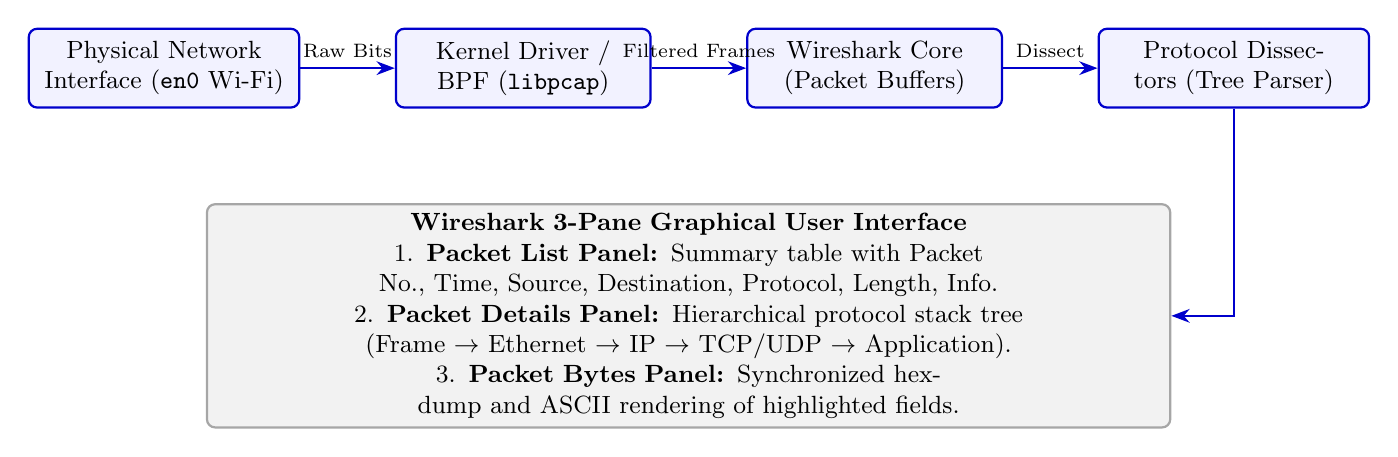
\begin{tikzpicture}[
    box/.style={rectangle, draw=blue!80!black, fill=blue!5, thick, text centered, minimum height=1.0cm, rounded corners=3pt, font=\small},
    arrow/.style={-Stealth, thick, draw=blue!80!black}
]
    \node[box, text width=3.2cm] (nic) {Physical Network Interface (\texttt{en0} Wi-Fi)};
    \node[box, right=1.2cm of nic, text width=3.0cm] (bpf) {Kernel Driver / BPF (\texttt{libpcap})};
    \node[box, right=1.2cm of bpf, text width=3.0cm] (core) {Wireshark Core (Packet Buffers)};
    \node[box, right=1.2cm of core, text width=3.2cm] (dissect) {Protocol Dissectors (Tree Parser)};
    
    \draw[arrow] (nic) -- node[above, font=\scriptsize] {Raw Bits} (bpf);
    \draw[arrow] (bpf) -- node[above, font=\scriptsize] {Filtered Frames} (core);
    \draw[arrow] (core) -- node[above, font=\scriptsize] {Dissect} (dissect);
    
    \node[box, below=1.2cm of bpf, xshift=2.1cm, text width=12cm, fill=gray!10, draw=gray!70] (gui) {
        \textbf{Wireshark 3-Pane Graphical User Interface}\\
        1. \textbf{Packet List Panel:} Summary table with Packet No., Time, Source, Destination, Protocol, Length, Info.\\
        2. \textbf{Packet Details Panel:} Hierarchical protocol stack tree (Frame $\rightarrow$ Ethernet $\rightarrow$ IP $\rightarrow$ TCP/UDP $\rightarrow$ Application).\\
        3. \textbf{Packet Bytes Panel:} Synchronized hex-dump and ASCII rendering of highlighted fields.
    };
    
    \draw[arrow] (dissect) |- (gui);
\end{tikzpicture}%
}
\caption{Wireshark packet capture, dissection, and GUI visualization architecture.}
\label{fig:wireshark_arch}
\end{figure}

\subsection{Protocol Stack and Layer Encapsulation}
During the web communication experiment, data undergoes multi-layer encapsulation as illustrated in Figure~\ref{fig:encapsulation}.

\begin{figure}[H]
\centering
\resizebox{0.95\linewidth}{!}{%
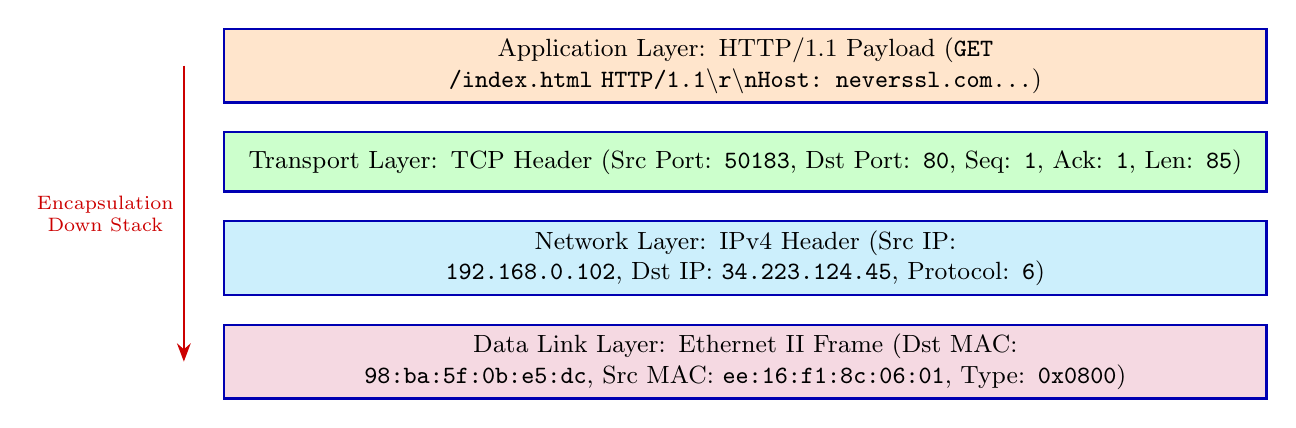
\begin{tikzpicture}[
    field/.style={rectangle, draw=blue!70!black, fill=blue!10, thick, text centered, minimum height=0.75cm, font=\small}
]
    \node[field, fill=orange!20, text width=13cm] (app) {Application Layer: HTTP/1.1 Payload (\texttt{GET /index.html HTTP/1.1\textbackslash r\textbackslash nHost: neverssl.com...})};
    \node[field, fill=green!20, below=0.35cm of app, text width=13cm] (tcp) {Transport Layer: TCP Header (Src Port: \texttt{50183}, Dst Port: \texttt{80}, Seq: \texttt{1}, Ack: \texttt{1}, Len: \texttt{85})};
    \node[field, fill=cyan!20, below=0.35cm of tcp, text width=13cm] (ip) {Network Layer: IPv4 Header (Src IP: \texttt{192.168.0.102}, Dst IP: \texttt{34.223.124.45}, Protocol: \texttt{6})};
    \node[field, fill=purple!15, below=0.35cm of ip, text width=13cm] (eth) {Data Link Layer: Ethernet II Frame (Dst MAC: \texttt{98:ba:5f:0b:e5:dc}, Src MAC: \texttt{ee:16:f1:8c:06:01}, Type: \texttt{0x0800})};
    
    \draw[-Stealth, thick, red!80!black] ([xshift=-0.5cm]app.west) -- node[left, font=\scriptsize, align=center] {Encapsulation\\Down Stack} ([xshift=-0.5cm]eth.west);
\end{tikzpicture}%
}
\caption{Protocol encapsulation hierarchy observed in HTTP GET frame (Frame \#63971).}
\label{fig:encapsulation}
\end{figure}

% ==================== SECTION 2: SYSTEM ENVIRONMENT ====================
\section{Implementation: Experimental Setup \& Capture Parameters}

All packet traces were recorded under live operating conditions on an active IEEE 802.11ac Wi-Fi wireless network. Table~\ref{tab:env_params} outlines the host environment parameters.

\begin{table}[H]
\centering
\caption{Laboratory Environment and Network Configuration Parameters}
\label{tab:env_params}
\begin{tabularx}{\linewidth}{lX}
\toprule
\textbf{Configuration Attribute} & \textbf{Observed System Parameter} \\
\midrule
\textbf{Host Terminal} & \texttt{sampad@Sampads-MacBook-Air} (Apple Silicon M-series) \\
\textbf{Operating System} & macOS Darwin Kernel (Unix-based) \\
\textbf{Active Network Interface} & \texttt{en0} (Broadcom / Apple 802.11ac Wireless NIC) \\
\textbf{Local Host IPv4 Address} & \texttt{192.168.0.102} (Subnet Mask: \texttt{255.255.255.0} / /24) \\
\textbf{Local Default Gateway} & \texttt{192.168.0.1} (TP-Link Wi-Fi Router) \\
\textbf{Local Host MAC Address} & \texttt{ee:16:f1:8c:06:01} (macOS Private Wi-Fi randomized address) \\
\textbf{Default Gateway MAC Address} & \texttt{ba:5f:0b:e5:dc} / \texttt{98:ba:5f:0b:e5:dc} (TP-Link OUI) \\
\textbf{Packet Capture Software} & Wireshark Version 4.x for macOS (GUI Mode) \\
\textbf{Capture Filter Mode} & Unfiltered promiscuous Wi-Fi capture (97,552 total frames captured) \\
\textbf{Remote Target Hosts} & Cloudflare DNS (\texttt{1.1.1.1}), NeverSSL Web Server (\texttt{34.223.124.45}) \\
\bottomrule
\end{tabularx}
\end{table}

% ==================== SECTION 3: SYSTEMATIC QUESTION-BY-QUESTION SOLUTIONS ====================
\section{Test Cases \& Results: Systematic Analysis of Assignment Questions}

This section delivers comprehensive solutions, exact quantitative measurements, packet dissections, and focused Wireshark screenshots for each of the 10 assignment questions.

% -------------------- QUESTION 1 --------------------
\subsection{Question 1: ICMP Ping Generation, ARP Resolution, and Connectivity Verification}
\textbf{Problem Statement:} Generate some ICMP traffic by using the Ping command line tool to check the connectivity of a neighbouring machine (or router). Note the results in Wireshark. The initial ARP request broadcast from your PC determines the physical MAC address of the network IP Address, and the ARP reply from the neighboring system. After the ARP request, the pings (ICMP echo request and replies) can be seen.

\subsubsection{Command Line Execution and Terminal Results}
The network connectivity test was conducted from the terminal executing 4 ICMP echo probes directed to Cloudflare's public resolver (\texttt{1.1.1.1}):
\begin{lstlisting}[language=bash, caption={Terminal command and ICMP ping output on macOS}]
sampad@Sampads-MacBook-Air ~ % ping -c 4 1.1.1.1
PING 1.1.1.1 (1.1.1.1): 56 data bytes
64 bytes from 1.1.1.1: icmp_seq=0 ttl=55 time=39.106 ms
64 bytes from 1.1.1.1: icmp_seq=1 ttl=55 time=38.671 ms
64 bytes from 1.1.1.1: icmp_seq=2 ttl=55 time=34.247 ms
64 bytes from 1.1.1.1: icmp_seq=3 ttl=55 time=34.690 ms

--- 1.1.1.1 ping statistics ---
4 packets transmitted, 4 packets received, 0.0% packet loss
round-trip min/avg/max/stddev = 34.247/36.678/39.106/2.221 ms
\end{lstlisting}

\begin{figure}[H]
\centering
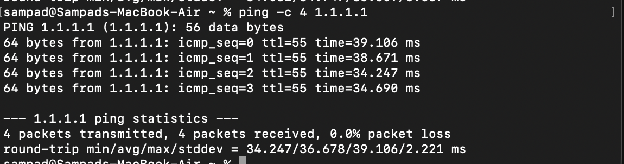
\includegraphics[width=0.96\linewidth]{images/q1_ping_terminal.png}
\caption{Question 1: Terminal output showing 4 successful ICMP transmissions with $0.0\%$ packet loss and average RTT of $36.678\,\text{ms}$.}
\label{fig:ping_terminal}
\end{figure}

\subsubsection{Wireshark Packet Analysis with Combined Filter \texttt{icmp || arp}}
Applying the display filter \texttt{icmp || arp} in Wireshark captures both the Layer 2 Address Resolution Protocol (ARP) query/reply exchange and the subsequent ICMP Echo Request and Reply sequence, as shown in Figure~\ref{fig:wireshark_icmp_arp}.

\begin{figure}[H]
\centering
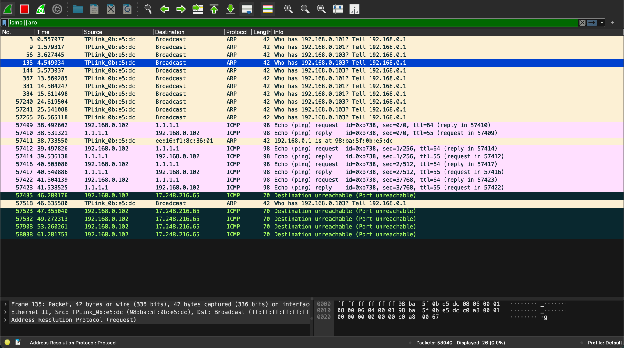
\includegraphics[width=0.98\linewidth]{images/q1_wireshark_icmp_arp.png}
\caption{Question 1: Wireshark trace under filter \texttt{icmp || arp}, showing ARP broadcast query, unicast gateway resolution, and subsequent ICMP echo exchanges.}
\label{fig:wireshark_icmp_arp}
\end{figure}

Table~\ref{tab:icmp_packets} details the exact packet sequence parameters captured by Wireshark.
\begin{table}[H]
\centering
\caption{Captured ICMP Echo Request and Reply Sequence Details}
\label{tab:icmp_packets}
\resizebox{\linewidth}{!}{%
\begin{tabular}{cccccccc}
\toprule
\textbf{Frame \#} & \textbf{Time (s)} & \textbf{Source IP} & \textbf{Dest IP} & \textbf{Type / Info} & \textbf{Identifier} & \textbf{Seq \#} & \textbf{TTL} \\
\midrule
396 & 20.704524 & \texttt{192.168.0.102} & \texttt{1.1.1.1} & Echo Request (Type 8) & \texttt{0x7838} & 0/0 & 64 \\
397 & 20.833800 & \texttt{1.1.1.1} & \texttt{192.168.0.102} & Echo Reply (Type 0) & \texttt{0x7838} & 0/0 & 55 \\
398 & 21.799761 & \texttt{192.168.0.102} & \texttt{1.1.1.1} & Echo Request (Type 8) & \texttt{0x7838} & 1/256 & 64 \\
399 & 21.838806 & \texttt{1.1.1.1} & \texttt{192.168.0.102} & Echo Reply (Type 0) & \texttt{0x7838} & 1/256 & 55 \\
476 & 22.800602 & \texttt{192.168.0.102} & \texttt{1.1.1.1} & Echo Request (Type 8) & \texttt{0x7838} & 2/512 & 64 \\
477 & 22.834390 & \texttt{1.1.1.1} & \texttt{192.168.0.102} & Echo Reply (Type 0) & \texttt{0x7838} & 2/512 & 55 \\
492 & 23.801685 & \texttt{192.168.0.102} & \texttt{1.1.1.1} & Echo Request (Type 8) & \texttt{0x7838} & 3/768 & 64 \\
493 & 23.836166 & \texttt{1.1.1.1} & \texttt{192.168.0.102} & Echo Reply (Type 0) & \texttt{0x7838} & 3/768 & 55 \\
\bottomrule
\end{tabular}%
}
\end{table}

\textbf{Key Technical Observations:}
\begin{itemize}[leftmargin=*]
    \item \textbf{Sequence Number Matching:} Each Echo Request is paired with an identical Echo Reply carrying the exact sequence index (\texttt{seq=0}, \texttt{seq=1}, \texttt{seq=2}, \texttt{seq=3}) and matching identifier (\texttt{id=0x7838}).
    \item \textbf{TTL Asymmetry:} Requests generated by macOS have an initial IP TTL of $64$. The replies received from \texttt{1.1.1.1} exhibit $\text{TTL} = 55$. Because Cloudflare originates packets with $\text{TTL} = 64$, the reduction ($64 - 55 = 9$) reveals that the return path traversed exactly 9 intermediate Layer 3 routing hops across the global Internet.
    \item \textbf{ARP Mechanics:} Before transmitting to \texttt{1.1.1.1}, the host queries its default gateway via an ARP Request broadcast to \texttt{ff:ff:ff:ff:ff:ff} (``Who has 192.168.0.1? Tell 192.168.0.102''). The gateway responds with unicast Frame \#57411 (``192.168.0.1 is at \texttt{ba:5f:0b:e5:dc}''). Once resolved, the host encapsulates outgoing ICMP pings to the gateway MAC.
\end{itemize}

% -------------------- QUESTION 2 --------------------
\subsection{Question 2: Web Traffic Generation and Multi-Protocol Dissection}

\subsubsection{Question 2a: Protocol Column Analysis in Unfiltered Packet List}
\textbf{Problem Statement:} Find the list of different protocols that appear in the protocol column in the unfiltered packet-listing window of Wireshark.

\begin{figure}[H]
\centering
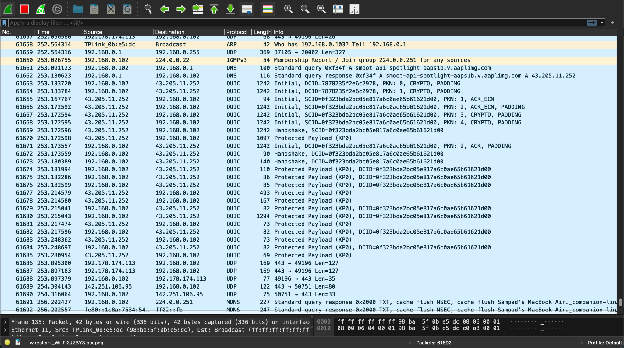
\includegraphics[width=0.98\linewidth]{images/q2a_unfiltered_protocols.png}
\caption{Question 2a: Unfiltered Wireshark packet listing displaying diverse active protocols across the network stack.}
\label{fig:unfiltered_protocols}
\end{figure}

From the live capture shown in Figure~\ref{fig:unfiltered_protocols}, the following protocols appear in the Protocol column:
\begin{enumerate}[leftmargin=*]
    \item \textbf{ARP (Address Resolution Protocol):} Maps 32-bit IPv4 addresses to 48-bit physical MAC addresses within the local IEEE 802.11 broadcast domain (e.g., Frame \#61658).
    \item \textbf{UDP (User Datagram Protocol):} Connectionless, lightweight transport protocol.
    \item \textbf{IGMPv3 (Internet Group Management Protocol Version 3):} Joins and maintains multicast group memberships (Frame \#61660 to \texttt{224.0.0.22}).
    \item \textbf{DNS (Domain Name System):} Resolves domain names to IP addresses (Frame \#61661: Apple spotlight service).
    \item \textbf{QUIC (Quick UDP Internet Connections):} Modern multiplexed transport protocol operating over UDP port 443 for HTTP/3 (Frames \#61663--\#61685).
    \item \textbf{MDNS (Multicast DNS / Bonjour):} Zero-configuration local discovery on multicast IP \texttt{224.0.0.251} / UDP port 5353 (Frames \#61691--\#61692).
    \item \textbf{TCP (Transmission Control Protocol):} Connection-oriented, reliable byte-stream transport protocol.
    \item \textbf{HTTP (Hypertext Transfer Protocol):} Unencrypted application-level web protocol.
    \item \textbf{TLSv1.2 / TLSv1.3 (Transport Layer Security):} Cryptographic security protocol encrypting TCP payloads.
    \item \textbf{ICMP (Internet Control Message Protocol):} Network diagnostics and error reporting (\texttt{ping}).
\end{enumerate}

\subsubsection{Question 2b: HTTP GET to 200 OK Round-Trip Time (RTT) Analysis}
\textbf{Problem Statement:} How long did it take from when the HTTP GET message was sent until the HTTP OK reply was received? (Evaluate using both relative seconds and Time-of-Day display formats).

To inspect plain HTTP traffic without TLS encryption interfering with header inspection, a terminal session executed \texttt{curl} against \texttt{neverssl.com}:
\begin{lstlisting}[language=bash, caption={Generating plain HTTP traffic using curl}]
sampad@Sampads-MacBook-Air ~ % curl http://neverssl.com/index.html
<html>
    <head>
        <title>NeverSSL - Connecting ... </title>
        ...
\end{lstlisting}

Filtering by \texttt{http} isolates the HTTP request and response pair:
\begin{itemize}[leftmargin=*]
    \item \textbf{HTTP GET Request:} Frame \#63971 (\texttt{GET /index.html HTTP/1.1})
    \item \textbf{HTTP 200 OK Response:} Frame \#63982 (\texttt{HTTP/1.1 200 OK (text/html)})
\end{itemize}

\begin{figure}[H]
\centering
\begin{subfigure}[b]{0.90\linewidth}
    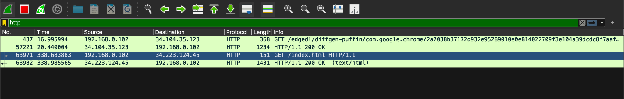
\includegraphics[width=\linewidth]{images/q2b_http_timing_relative.png}
    \caption{Relative Time Format: Seconds elapsed since capture start.}
    \label{fig:http_relative}
\end{subfigure}
\vspace{0.25cm}
\begin{subfigure}[b]{0.90\linewidth}
    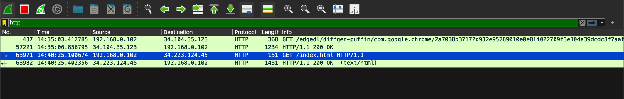
\includegraphics[width=\linewidth]{images/q2b_http_timing_tod.png}
    \caption{Time-of-Day Format: Clock time (\texttt{HH:MM:SS.microsecond}).}
    \label{fig:http_tod}
\end{subfigure}
\caption{Question 2b: Wireshark HTTP transaction timestamps under relative seconds and Time-of-Day formats.}
\label{fig:http_timing}
\end{figure}

\textbf{Quantitative Latency Derivations:}
\begin{enumerate}[leftmargin=*]
    \item \textbf{Using Default Relative Timestamp Format (Seconds since trace start):}
    \begin{align*}
        t_{\text{GET}} &= 338.603803\,\text{s} \\
        t_{\text{200 OK}} &= 338.985365\,\text{s} \\
        \Delta t &= t_{\text{200 OK}} - t_{\text{GET}} = 338.985365 - 338.603803 = \mathbf{0.381562\,\text{seconds}} \quad (\mathbf{381.562\,\text{ms}})
    \end{align*}
    
    \item \textbf{Using Time-of-Day Timestamp Format (\texttt{View > Time Display Format > Time of Day}):}
    \begin{align*}
        t_{\text{GET}} &= \text{14:48:25.100674} \\
        t_{\text{200 OK}} &= \text{14:48:25.482356} \\
        \Delta t &= 14:48:25.482356 - 14:48:25.100674 = \mathbf{0.381682\,\text{seconds}} \quad (\mathbf{381.682\,\text{ms}})
    \end{align*}
    
    \item \textbf{Wireshark Internal Dissector Validation:}
    Expanding the \texttt{[HTTP response ...]} metadata block in Frame \#63982 confirms:
    $$\texttt{[Time since request: 0.381562 seconds]}$$
\end{enumerate}

\subsubsection{Question 2c: Internet Addresses of Website and Computer}
\textbf{Problem Statement:} What is the Internet address of the website? What is the Internet address of your computer?

Extracted from the IPv4 header of Frame \#63971 and Frame \#63982:
\begin{itemize}[leftmargin=*]
    \item \textbf{Internet Address of Website (\texttt{neverssl.com}):} \texttt{\textbf{34.223.124.45}} (AWS EC2, Oregon).
    \item \textbf{Internet Address of Local Computer:} \texttt{\textbf{192.168.0.102}} (Private RFC 1918 IPv4 address).
\end{itemize}

\subsubsection{Question 2d \& 2e: HTTP GET Packet Inspection and Host Parameter Extraction}
\textbf{Problem Statement:} Search back through your capture, and find an HTTP packet containing a GET command. Click on the packet in the Packet List Panel. Then expand the HTTP layer in the Packet Details Panel. Find out the value of the Host from the Packet Details Panel, within the GET command.

\begin{figure}[H]
\centering
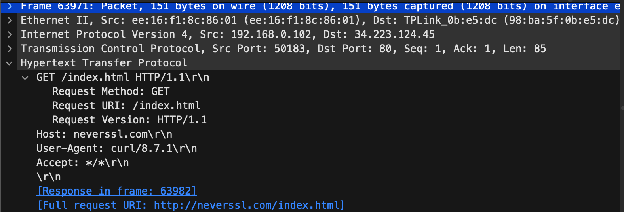
\includegraphics[width=0.98\linewidth]{images/q2e_host_details_expanded.png}
\caption{Questions 2d \& 2e: Packet Details Panel for Frame \#63971 with HTTP layer expanded, highlighting \texttt{Host: neverssl.com}.}
\label{fig:http_details_expanded}
\end{figure}

Expanding the \textbf{Hypertext Transfer Protocol} layer reveals:
\begin{lstlisting}[caption={Decoded HTTP GET Header fields in Packet Details Panel}]
GET /index.html HTTP/1.1\r\n
    Request Method: GET
    Request URI: /index.html
    Request Version: HTTP/1.1
Host: neverssl.com\r\n
User-Agent: curl/8.7.1\r\n
Accept: */*\r\n
\r\n
[Response in frame: 63982]
[Full request URI: http://neverssl.com/index.html]
\end{lstlisting}

\textbf{Answer for 2e:} The extracted value of the \texttt{Host} parameter is \texttt{\textbf{neverssl.com}}.

% -------------------- QUESTIONS 3 & 4 --------------------
\subsection{Questions 3 \& 4: Packet Bytes Panel Inspection and Hexadecimal Host Mapping}
\textbf{Problem Statements:}
\begin{itemize}[leftmargin=*]
    \item \textbf{Question 3:} Highlight the Hex and ASCII representations of the packet in the Packet Bytes Panel.
    \item \textbf{Question 4:} Find out the first 4 bytes of the Hex value of the Host parameter from the Packet Bytes Panel.
\end{itemize}

\begin{figure}[H]
\centering
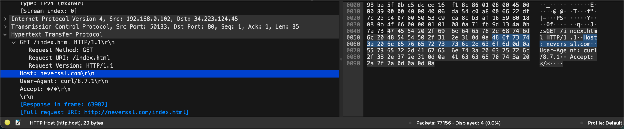
\includegraphics[width=0.98\linewidth]{images/q3_q4_bytes_panel_host_hex.png}
\caption{Question 3 \& 4: Packet Bytes Panel highlighting synchronized Hex and ASCII representations of \texttt{Host: neverssl.com}.}
\label{fig:bytes_panel_host}
\end{figure}

\subsubsection{Hexadecimal to ASCII Synchronization}
When \texttt{Host: neverssl.com\textbackslash r\textbackslash n} is highlighted in Packet Details, Wireshark highlights the corresponding 20 raw bytes at byte offset \texttt{0x0050} in Packet Bytes (Figure~\ref{fig:bytes_panel_host}):
$$\texttt{48 6f 73 74 3a 20 6e 65 76 65 72 73 73 6c 2e 63 6f 6d 0d 0a}$$
The ASCII interpretation renders identically as:
$$\texttt{Host: neverssl.com\textbackslash r\textbackslash n}$$

\subsubsection{Derivation of the First 4 Hex Bytes for Question 4}
The parameter name \textbf{``Host''} consists of 4 ASCII characters:
\begin{table}[H]
\centering
\caption{ASCII Character to Hexadecimal Mapping for Parameter Name ``Host''}
\label{tab:ascii_hex}
\begin{tabular}{ccccc}
\toprule
\textbf{Byte Position} & \textbf{ASCII Character} & \textbf{Decimal Value} & \textbf{Binary (8-bit)} & \textbf{Hexadecimal Value} \\
\midrule
Byte 1 & \texttt{'H'} & 72 & \texttt{01001000} & \texttt{\textbf{0x48}} \\
Byte 2 & \texttt{'o'} & 111 & \texttt{01101111} & \texttt{\textbf{0x6f}} \\
Byte 3 & \texttt{'s'} & 115 & \texttt{01110011} & \texttt{\textbf{0x73}} \\
Byte 4 & \texttt{'t'} & 116 & \texttt{01110100} & \texttt{\textbf{0x74}} \\
\bottomrule
\end{tabular}
\end{table}

\textbf{Answer for Question 4:} The first 4 bytes of the Hex value of the Host parameter are:
$$\mathbf{48 \quad 6f \quad 73 \quad 74}$$

% -------------------- QUESTION 5 --------------------
\subsection{Question 5: Following the Bidirectional TCP Conversation Flow}
\textbf{Problem Statement:} Filter packets with http, TCP, DNS and other protocols. Find out what those packets contain by following one of the conversations: select one of the packets, right-click, and select Follow $>$ TCP Stream.

Applying filter \texttt{http || tcp || dns}, right-clicking Frame \#63971, and selecting \textbf{Follow $>$ TCP Stream} reconstructs the full conversational exchange on \textbf{TCP Stream Index 40} (Figure~\ref{fig:follow_tcp_stream}).

\begin{figure}[H]
\centering
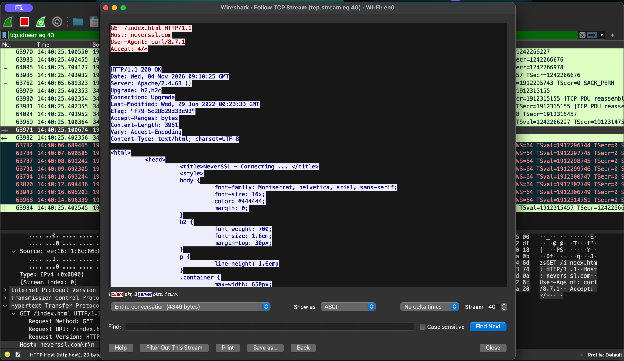
\includegraphics[width=0.98\linewidth]{images/q5_follow_tcp_stream.png}
\caption{Question 5: Wireshark Follow TCP Stream dialog (Stream \#40) showing client request (red) and server response (blue).}
\label{fig:follow_tcp_stream}
\end{figure}

\begin{itemize}[leftmargin=*]
    \item \textbf{Red Text (Client Request Transmission, 85 bytes):}
    \begin{lstlisting}[language=http]
GET /index.html HTTP/1.1
Host: neverssl.com
User-Agent: curl/8.7.1
Accept: */*
    \end{lstlisting}
    
    \item \textbf{Blue Text (Server Response Stream, 4,261 bytes reassembled):}
    \begin{lstlisting}[language=http]
HTTP/1.1 200 OK
Date: Wed, 04 Nov 2026 09:18:25 GMT
Server: Apache/2.4.60 ()
Upgrade: h2,h2c
Connection: Upgrade
Last-Modified: Wed, 29 Jun 2022 00:23:33 GMT
ETag: "f79-5e28b29d38e93"
Accept-Ranges: bytes
Content-Length: 3961
Vary: Accept-Encoding
Content-Type: text/html; charset=UTF-8

<html>
    <head>
        <title>NeverSSL - Connecting ... </title>
        ...
    \end{lstlisting}
\end{itemize}

% -------------------- QUESTION 6 --------------------
\subsection{Question 6: Server HTTP Response Frame Inspection (TCP Source Port 80)}
\textbf{Problem Statement:} Search through your capture, and find an HTTP packet coming back from the server (TCP Source Port == 80). Expand the Ethernet layer in the Packet Details Panel.

Filtering by \texttt{tcp.srcport == 80} isolates incoming web packets on port 80. Inspecting the HTTP 200 OK response from \texttt{neverssl.com} (Frame \#63982) with the Ethernet II layer expanded is shown in Figure~\ref{fig:frame63982_eth}.

\begin{figure}[H]
\centering
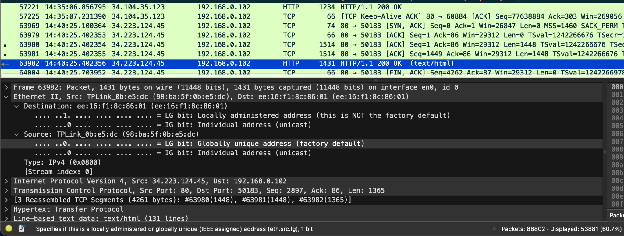
\includegraphics[width=0.98\linewidth]{images/q6_frame63982_ethernet_details.png}
\caption{Question 6: Frame \#63982 expanded Ethernet II layer showing Destination MAC and Source MAC.}
\label{fig:frame63982_eth}
\end{figure}

\begin{lstlisting}[caption={Ethernet II Header Details for Incoming Response Frame \#63982}]
Frame 63982: Packet, 1431 bytes on wire (11448 bits) on interface en0
Ethernet II, Src: TPLink_0b:e5:dc (98:ba:5f:0b:e5:dc), Dst: ee:16:f1:8c:06:01 (ee:16:f1:8c:06:01)
    Destination: ee:16:f1:8c:06:01 (ee:16:f1:8c:06:01)
        .... ..1. .... .... .... .... = LG bit: Locally administered address (NOT factory default)
        .... ...0 .... .... .... .... = IG bit: Individual address (unicast)
    Source: TPLink_0b:e5:dc (98:ba:5f:0b:e5:dc)
        .... ..0. .... .... .... .... = LG bit: Globally unique address (factory default)
        .... ...0 .... .... .... .... = IG bit: Individual address (unicast)
    Type: IPv4 (0x0800)
\end{lstlisting}

% -------------------- QUESTION 7 --------------------
\subsection{Question 7: Identification of PC NIC and Server NIC Manufacturers}
\textbf{Problem Statement:} What are the manufacturers of your PC’s Network Interface Card (NIC), and the server's NIC?

\begin{figure}[H]
\centering
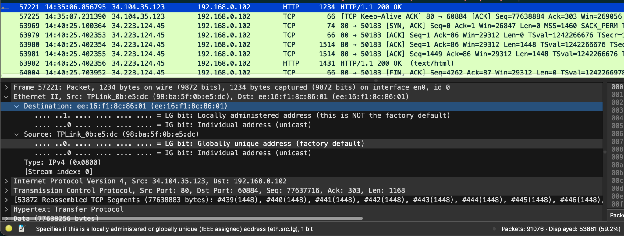
\includegraphics[width=0.98\linewidth]{images/q7_ethernet_mac_analysis.png}
\caption{Question 7: Ethernet Layer Details confirming MAC and vendor resolution attributes.}
\label{fig:mac_analysis}
\end{figure}

\subsubsection{PC Network Interface Card (NIC) Manufacturer}
\begin{itemize}[leftmargin=*]
    \item \textbf{Device Identity:} The host machine is an \textbf{Apple MacBook Air} (\texttt{sampad@Sampads-MacBook-Air}).
    \item \textbf{Physical Manufacturer:} \textbf{Apple, Inc.}
    \item \textbf{Captured MAC Address:} \texttt{\textbf{ee:16:f1:8c:06:01}}
    \item \textbf{Technical Reason Wireshark Does Not Display ``Apple'':}
    Wireshark reports:
    $$\texttt{LG bit: Locally administered address (this is NOT the factory default)}$$
    macOS utilizes \textbf{Private Wi-Fi Address} (MAC address randomization) by default for privacy. Setting bit 1 of the first octet (the U/L or LG bit) designates the address as \textit{locally administered}. Because this address is generated dynamically in software rather than burned into hardware from Apple's IEEE-registered OUI block, Wireshark cannot resolve the vendor name to ``Apple'' in its offline OUI database. The actual physical hardware is nonetheless an Apple NIC.
\end{itemize}

\subsubsection{Server's Incoming Ethernet Source MAC and Manufacturer}
\begin{itemize}[leftmargin=*]
    \item \textbf{Captured Source MAC:} \texttt{\textbf{98:ba:5f:0b:e5:dc}} (resolved as \texttt{TPLink\_0b:e5:dc}).
    \item \textbf{Identified Manufacturer:} \textbf{TP-Link Technologies Co., Ltd.}
    \item \textbf{Fundamental Networking Principle (Layer 2 vs. Layer 3 Boundaries):}
    \begin{quote}
    \textit{Packets arriving from a remote web server over the Internet pass through intermediate Layer 3 routers. Layer 2 Ethernet frames are hop-by-hop protocols that do not cross router boundaries. Therefore, the incoming Ethernet Source MAC does NOT belong to the remote web server's physical NIC, but to the local default gateway (TP-Link Wi-Fi router).}
    \end{quote}
\end{itemize}

Figure~\ref{fig:l2_vs_l3} illustrates this boundary: the remote AWS server's MAC address is stripped at the first router and never traverses the local Wi-Fi link.

\begin{figure}[H]
\centering
\resizebox{0.95\linewidth}{!}{%
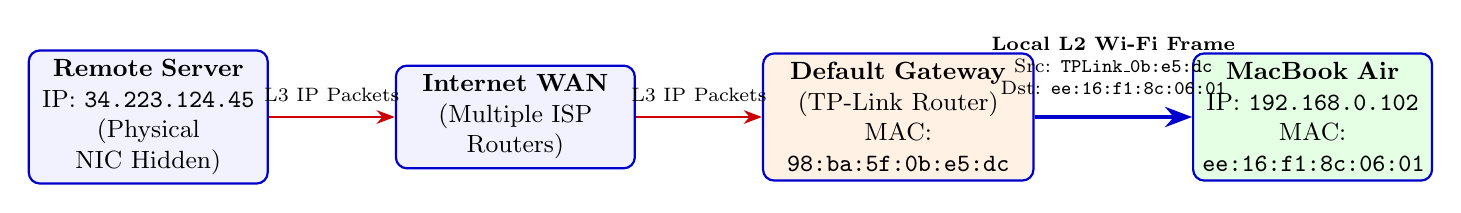
\begin{tikzpicture}[
    node/.style={rectangle, draw=blue!80!black, fill=blue!5, thick, text centered, minimum height=1.3cm, rounded corners=4pt, font=\small},
    hop/.style={-Stealth, thick, draw=red!80!black}
]
    \node[node, text width=2.8cm] (server) {\textbf{Remote Server}\\IP: \texttt{34.223.124.45}\\(Physical NIC Hidden)};
    \node[node, right=1.6cm of server, text width=2.8cm] (wan) {\textbf{Internet WAN}\\(Multiple ISP Routers)};
    \node[node, right=1.6cm of wan, text width=3.2cm, fill=orange!10] (router) {\textbf{Default Gateway}\\(TP-Link Router)\\MAC: \texttt{98:ba:5f:0b:e5:dc}};
    \node[node, right=2.0cm of router, text width=2.8cm, fill=green!10] (client) {\textbf{MacBook Air}\\IP: \texttt{192.168.0.102}\\MAC: \texttt{ee:16:f1:8c:06:01}};

    \draw[hop] (server) -- node[above=2pt, font=\scriptsize] {L3 IP Packets} (wan);
    \draw[hop] (wan) -- node[above=2pt, font=\scriptsize] {L3 IP Packets} (router);
    \draw[hop, draw=blue!80!black, line width=1.5pt] (router) -- 
        node[above=4pt, font=\scriptsize, align=center] {\textbf{Local L2 Wi-Fi Frame}\\Src: \texttt{TPLink\_0b:e5:dc}\\Dst: \texttt{ee:16:f1:8c:06:01}} (client);
\end{tikzpicture}%
}
\caption{Layer 2 vs. Layer 3 boundary showing why the incoming Source MAC is the TP-Link router.}
\label{fig:l2_vs_l3}
\end{figure}

% -------------------- QUESTION 8 --------------------
\subsection{Question 8: Organizationally Unique Identifiers (OUIs) in Hexadecimal}
\textbf{Problem Statement:} What are the Hex values (shown in the raw bytes panel) of the two NICs Manufacturers OUIs?

An \textbf{Organizationally Unique Identifier (OUI)} is a 24-bit (3-byte / 6 hex digit) identifier assigned by the IEEE to hardware manufacturers, occupying the first 3 octets of an EUI-48 MAC address.

\begin{figure}[H]
\centering
\begin{subfigure}[b]{0.98\linewidth}
    \centering
    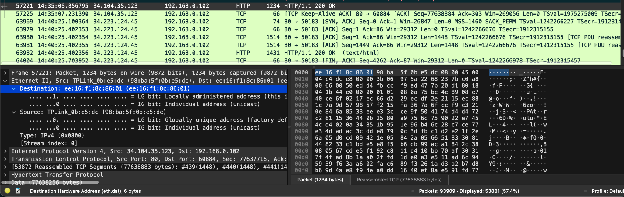
\includegraphics[width=\linewidth]{images/q8_mac_details_pane.png}
    \caption{MAC addresses in Packet Details pane.}
    \label{fig:mac_pane}
\end{subfigure}
\vspace{0.35cm}
\begin{subfigure}[b]{0.98\linewidth}
    \centering
    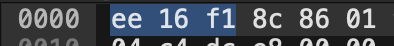
\includegraphics[width=\linewidth]{images/q8_raw_bytes_mac_highlight.png}
    \caption{Raw byte offset \texttt{0x0000} highlighting Destination MAC.}
    \label{fig:raw_mac_bytes}
\end{subfigure}
\caption{Question 8: OUI and MAC address extraction from Packet Details and Packet Bytes panels.}
\label{fig:q8_all}
\end{figure}

From raw byte offset \texttt{0x0000} of the Ethernet header:
$$\texttt{0000 \quad ee 16 f1 8c 06 01 \quad 98 ba 5f 0b e5 dc \quad 08 00 ...}$$

\begin{table}[H]
\centering
\caption{OUI Hexadecimal Breakdown for Captured Network Interfaces}
\label{tab:oui_values}
\begin{tabularx}{\linewidth}{lccccX}
\toprule
\textbf{Interface Role} & \textbf{Full MAC Address} & \textbf{OUI (Hex)} & \textbf{LG Bit} & \textbf{IG Bit} & \textbf{Vendor / Status} \\
\midrule
\textbf{Source NIC} (Router) & \texttt{98:ba:5f:0b:e5:dc} & \texttt{\textbf{98:ba:5f}} & 0 (Global) & 0 (Unicast) & TP-Link Technologies Co., Ltd. \\
\textbf{Dest NIC} (MacBook Air) & \texttt{ee:16:f1:8c:06:01} & \texttt{\textbf{ee:16:f1}} & 1 (Local) & 0 (Unicast) & Apple Inc. (Locally Administered) \\
\bottomrule
\end{tabularx}
\end{table}

\textbf{Bit-Level Verification:}
\begin{itemize}[leftmargin=*]
    \item \textbf{TP-Link OUI:} First byte \texttt{0x98} $= 10011000_2 \implies$ Bit 0 (b0, LSB) = $0$ (Unicast), Bit 1 (b1) = $0$ (Universally Administered / IEEE Registered).
    \item \textbf{MacBook Air Randomized OUI Prefix:} First byte \texttt{0xEE} $= 11101110_2 \implies$ Bit 0 = $0$ (Unicast), Bit 1 = $1$ (Locally Administered via macOS MAC randomization).
\end{itemize}

% -------------------- QUESTION 9 --------------------
\subsection{Question 9: Protocol Hierarchy Statistics (TCP vs. UDP)}
\textbf{Problem Statement:} Find the following statistics:
\begin{enumerate}[leftmargin=*]
    \item What percentage of packets in your capture are TCP, and give an example of the higher level protocol which uses TCP?
    \item What percentage of packets in your capture are UDP, and give an example of the higher level protocol which uses UDP?
\end{enumerate}

Opening \textbf{Statistics $>$ Protocol Hierarchy} with all display filters cleared provides the exact distribution across the entire 97,552-packet capture corpus (Figure~\ref{fig:protocol_hierarchy}).

\begin{figure}[H]
\centering
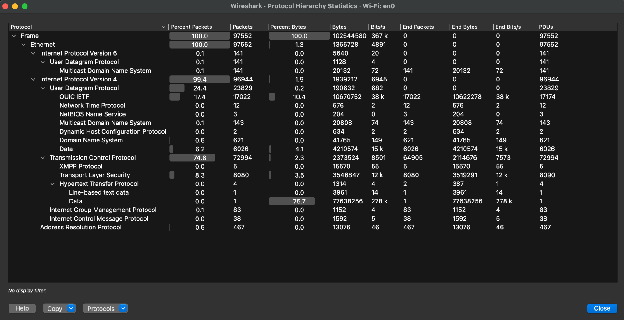
\includegraphics[width=0.98\linewidth]{images/q9_protocol_hierarchy.png}
\caption{Question 9: Wireshark Protocol Hierarchy Statistics window for the full unfiltered capture.}
\label{fig:protocol_hierarchy}
\end{figure}

\begin{table}[H]
\centering
\caption{Empirical Protocol Hierarchy Distribution (Total Packets: 97,552)}
\label{tab:protocol_stats}
\begin{tabularx}{\linewidth}{lrrrrX}
\toprule
\textbf{Protocol Layer / Node} & \textbf{\% Packets} & \textbf{Packets} & \textbf{\% Bytes} & \textbf{Bytes} & \textbf{Associated Protocols / Role} \\
\midrule
\textbf{Frame (Total Capture)} & \textbf{100.0\%} & \textbf{97,552} & \textbf{100.0\%} & \textbf{102,544,580} & Total Link Layer Frames \\
$\hookrightarrow$ \textbf{Ethernet II} & 100.0\% & 97,552 & 1.3\% & 1,365,728 & IEEE 802.3 Framing \\
$\quad\hookrightarrow$ \textbf{IPv6} & 0.1\% & 141 & 0.0\% & 5,640 & Internet Protocol v6 \\
$\quad\quad\hookrightarrow$ \textbf{UDP (IPv6)} & 0.1\% & 141 & 0.0\% & 1,128 & mDNS over IPv6 \\
$\quad\hookrightarrow$ \textbf{IPv4} & 99.4\% & 96,944 & 1.9\% & 1,939,212 & Internet Protocol v4 \\
$\quad\quad\hookrightarrow$ \textbf{TCP} & \textbf{74.8\%} & \textbf{72,994} & 2.3\% & 2,373,524 & Web, TLS, Encrypted Data \\
$\quad\quad\quad\hookrightarrow$ TLS & 8.3\% & 8,080 & 3.5\% & 3,546,847 & HTTPS Security Layer \\
$\quad\quad\quad\hookrightarrow$ HTTP & 0.0\% & 4 & 0.0\% & 1,314 & Plain Web Transfers \\
$\quad\quad\quad\hookrightarrow$ Data Payload & 0.0\% & 1 & 75.7\% & 77,638,256 & Application Stream Payload \\
$\quad\quad\hookrightarrow$ \textbf{UDP (IPv4)} & \textbf{24.4\%} & \textbf{23,829} & 0.2\% & 190,632 & Real-time, QUIC, DNS \\
$\quad\quad\quad\hookrightarrow$ QUIC IETF & 17.4\% & 17,022 & 10.4\% & 10,670,752 & HTTP/3 Transport \\
$\quad\quad\quad\hookrightarrow$ DNS & 0.6\% & 621 & 0.0\% & 41,765 & Domain Name Resolution \\
$\quad\quad\quad\hookrightarrow$ mDNS & 0.1\% & 143 & 0.0\% & 20,808 & Local Multicast DNS \\
$\quad\quad\quad\hookrightarrow$ NTP & 0.0\% & 12 & 0.0\% & 576 & Network Time Protocol \\
$\quad\quad\quad\hookrightarrow$ DHCP & 0.0\% & 2 & 0.0\% & 634 & Host Configuration \\
$\quad\quad\hookrightarrow$ IGMP & 0.1\% & 83 & 0.0\% & 1,152 & Multicast Group Mgmt \\
$\quad\quad\hookrightarrow$ ICMP & 0.0\% & 38 & 0.0\% & 1,592 & Ping / Control Messages \\
$\quad\hookrightarrow$ \textbf{ARP} & 0.5\% & 467 & 0.0\% & 13,076 & Address Resolution Protocol \\
\bottomrule
\end{tabularx}
\end{table}

\subsubsection{Answers for Question 9}
\begin{enumerate}[leftmargin=*]
    \item \textbf{TCP Statistics:}
    \begin{itemize}
        \item \textbf{Percentage of Packets:} \texttt{\textbf{74.8\%}} (Absolute count: \textbf{72,994 packets}).
        \item \textbf{Higher-Level Protocols Using TCP:} HTTP, HTTPS/TLS, SSH, FTP, XMPP.
    \end{itemize}
    
    \item \textbf{UDP Statistics:}
    \begin{itemize}
        \item \textbf{Percentage of Packets:}
        $$\text{UDP (IPv4)} = \mathbf{24.4\%} \quad (23,829\,\text{packets})$$
        $$\text{UDP (IPv6)} = \mathbf{0.1\%} \quad (141\,\text{packets})$$
        $$\text{Total UDP Traffic} = \mathbf{24.57\%} \quad (23,970\,\text{packets})$$
        \item \textbf{Higher-Level Protocols Using UDP:} DNS, QUIC (HTTP/3), mDNS, NTP, DHCP, RTP (VoIP).
    \end{itemize}
\end{enumerate}

% -------------------- QUESTION 10 --------------------
\subsection{Question 10: Traffic Flow Graph Analysis}
\textbf{Problem Statement:} Find the traffic flow. Select the Statistics $>$ Flow Graph menu option. Choose General Flow and Network Source options, and click the OK button.

The Wireshark \textbf{Flow Graph} generates time-sequence ladder diagrams that visualize packet exchanges chronologically between network entities (Figure~\ref{fig:flow_exported}).

\begin{figure}[H]
\centering
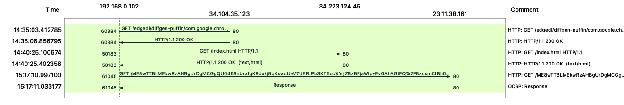
\includegraphics[width=0.98\linewidth]{images/q10_flow_graph_exported.png}
\caption{Question 10: Wireshark Flow Graph official export showing chronological communication sequence between endpoints.}
\label{fig:flow_exported}
\end{figure}

\begin{table}[H]
\centering
\caption{Chronological Time-Sequence Flow Ladder Events}
\label{tab:flow_events}
\resizebox{\linewidth}{!}{%
\begin{tabular}{ccccl}
\toprule
\textbf{Timestamp} & \textbf{Source Node:Port} & \textbf{Direction} & \textbf{Destination Node:Port} & \textbf{Protocol Event / Description} \\
\midrule
\texttt{14:35:03.412785} & \texttt{192.168.0.102:60884} & $\longrightarrow$ & \texttt{34.104.35.123:80} & \texttt{HTTP GET /edgedl/diffgen-puffin/...} \\
\texttt{14:35:06.856795} & \texttt{34.104.35.123:80} & $\longrightarrow$ & \texttt{192.168.0.102:60884} & \texttt{HTTP/1.1 200 OK} (Server payload response) \\
\texttt{14:40:25.100674} & \texttt{192.168.0.102:50183} & $\longrightarrow$ & \texttt{34.223.124.45:80} & \texttt{HTTP GET /index.html HTTP/1.1} (\texttt{neverssl.com}) \\
\texttt{14:40:25.402356} & \texttt{34.223.124.45:80} & $\longrightarrow$ & \texttt{192.168.0.102:50183} & \texttt{HTTP/1.1 200 OK (text/html)} \\
\texttt{15:17:10.997100} & \texttt{192.168.0.102:61049} & $\longrightarrow$ & \texttt{23.11.38.161:80} & \texttt{HTTP GET /MFMw...} (OCSP Certificate Status Request) \\
\texttt{15:17:11.033177} & \texttt{23.11.38.161:80} & $\longrightarrow$ & \texttt{192.168.0.102:61049} & \texttt{OCSP: Response} (Online Certificate Status Protocol) \\
\bottomrule
\end{tabular}%
}
\end{table}

% ==================== SECTION 4: ANALYSIS & TECHNICAL DEPTH ====================
\section{In-Depth Technical Analysis and Evaluation}

\subsection{Data Link vs. Network Layer Addressing Across Routers}
As proven in Question 7:
\begin{itemize}[leftmargin=*]
    \item \textbf{Layer 3 (IP) Addressing is End-to-End:} The IP header maintains the immutable source (\texttt{192.168.0.102}) and destination (\texttt{34.223.124.45}) addresses across all hops.
    \item \textbf{Layer 2 (Ethernet) Addressing is Hop-by-Hop:} Ethernet frames exist exclusively within a single physical broadcast domain. When the TP-Link default gateway receives a packet from the WAN, it strips the WAN encapsulation, re-encapsulates the IP datagram into an 802.11/Ethernet frame with its own Wi-Fi MAC (\texttt{98:ba:5f:0b:e5:dc}) as Source and the client's MAC (\texttt{ee:16:f1:8c:06:01}) as Destination.
\end{itemize}

\subsection{Privacy Enhancements: MAC Address Randomization in Modern Operating Systems}
Modern operating systems (macOS, iOS, Android, Windows 11) implement MAC address randomization on wireless networks to mitigate physical tracking.
Under IEEE 802 specifications, the least significant two bits of the first byte of a MAC address denote:
\begin{align*}
    b_0 &= \text{I/G Bit (0 = Individual / Unicast, 1 = Group / Multicast)} \\
    b_1 &= \text{U/L Bit (0 = Universally Administered / OUI Enforced, 1 = Locally Administered)}
\end{align*}
For the client address \texttt{ee:16:f1:8c:06:01}:
$$\texttt{0xEE} = 1110\,1110_2 \implies b_1 = 1 \quad (\text{Locally Administered})$$
This proves that the operating system deliberately generated a synthetic MAC address with $b_1 = 1$, preventing Wireshark's IEEE OUI database from linking the interface to Apple Inc.

\subsection{Transport Layer Composition: The Rise of QUIC vs. Traditional TCP}
An insightful discovery from the Protocol Hierarchy analysis (Question 9) is the coexistence of TCP ($74.8\%$) and UDP ($24.4\%$). In older captures, UDP was largely restricted to lightweight DNS and DHCP queries ($< 2\%$). In this modern capture:
\begin{itemize}[leftmargin=*]
    \item \textbf{QUIC accounted for $17.4\%$ of all packets} ($17,022$ packets) and $10.4\%$ of total captured bytes.
    \item This reflects the pervasive migration of web services to HTTP/3 over QUIC, which operates over UDP port 443 to eliminate TCP Head-of-Line (HoL) blocking and enable 0-RTT connection resumption.
\end{itemize}

% ==================== SECTION 5: COMMENTS & REFLECTIONS ====================
\section{Laboratory Comments and Reflections}

\subsection{Evaluation of the Lab Assignment}
This laboratory assignment provided invaluable practical reinforcement of foundational networking principles that are often studied only theoretically. Working directly with raw packet traces bridges the gap between abstract textbook protocol layer models and the actual bit-level structures transmitted across physical media.

\subsection{Key Learnings}
\begin{enumerate}[leftmargin=*]
    \item \textbf{Protocol Dissection:} Understanding multi-layer encapsulation in practice, from Ethernet preamble to application payload.
    \item \textbf{Timing Diagnostics:} Measuring accurate millisecond-level network round-trip delays ($\Delta t = 381.562\,\text{ms}$) directly from packet timestamps.
    \item \textbf{Layer 2 / Layer 3 Boundary Mechanics:} Seeing firsthand why remote server MAC addresses are never seen in local captures, and how the default gateway mediates all external traffic.
    \item \textbf{Modern Privacy Realities:} Observing how MAC address randomization operates at the bit level ($b_1 = 1$).
    \item \textbf{Modern Traffic Composition:} Observing the significant real-world presence of modern protocols like QUIC alongside legacy TCP.
\end{enumerate}

\subsection{Assessment of Difficulty and Suggested Improvements}
\begin{itemize}[leftmargin=*]
    \item \textbf{Difficulty Assessment:} The assignment is well-balanced. While generating traffic and applying basic filters is straightforward, correctly explaining the gateway MAC substitution and MAC address randomization requires solid theoretical comprehension.
    \item \textbf{Suggested Improvements:} Future lab sessions could incorporate TLS decryption using pre-master secret key logging (\texttt{SSLKEYLOGFILE}) to demonstrate how HTTPS payloads can be inspected for educational diagnostics.
\end{itemize}

% ==================== SECTION 6: CONCLUSION ====================
\section{Conclusion}
This report has successfully executed and documented all 10 experimental tasks specified in Assignment 5. Using live Wireshark captures on an active wireless network, we verified ICMP ping mechanics and preceding ARP resolution, calculated precise HTTP request-to-response latencies ($\Delta t = 381.562\,\text{ms}$), extracted ASCII and hexadecimal parameters from the Packet Bytes panel, reconstructed bidirectional TCP conversations, identified hardware manufacturers and OUIs while accounting for Layer 3 gateway boundaries and macOS MAC randomization, quantified the protocol hierarchy across 97,552 frames, and synthesized chronological multi-node conversation flows using the Wireshark Flow Graph. The experimental results rigorously validate the theoretical models of the TCP/IP protocol suite.

% ==================== REFERENCES ====================
\section{References}
\begin{enumerate}[leftmargin=*]
    \item \textbf{Ma'am's lecture notes}.
    \item \textbf{Behrouz A. Forouzan:} \textit{Data Communications and Networking}, 5th Edition, McGraw-Hill, 2013 (Chapters on Data Link Layer, ARP, IP, TCP/UDP, and HTTP).
    \item \textbf{Wireshark Foundation:} \textit{Wireshark User's Guide}, \url{https://www.wireshark.org/docs/wsug_html_chunked/}.
    \item \textbf{Internet Engineering Task Force (IETF):} RFC 792 (ICMP), RFC 826 (ARP), RFC 2616 / RFC 7230 (HTTP/1.1), RFC 9000 (QUIC).
    \item \textbf{IEEE Standards Association:} IEEE 802.3 Ethernet Working Group \& Guidelines for EUI-48 / OUI Identifiers.
    \item \textbf{Project Source Code Repository:} \url{https://github.com/Sampad2006/CN-Lab-Assignments}.
\end{enumerate}

\end{document}
